% Presentación del Curso de LaTeX preparado para 
% el ITVM, del 20 al 24 de enero del 2020
% Gerardo Marx Chávez-Campos 
%--------------------------------
\documentclass[gray]{beamer}
%\usetheme{Darmstadt}
\usetheme{Warsaw}
%\usecolortheme{seahorse}
\setbeamercovered{transparent}
%Librerías requeridas
\usepackage[spanish]{babel}
\usepackage[utf8]{inputenc}
\usepackage{graphicx}
\usepackage{hyperref}
\usepackage{color}
\usepackage{xcolor}
\usepackage{listings}
\usepackage[compatibility=false]{caption}
\DeclareCaptionFont{white}{\color{white}}
\DeclareCaptionFormat{listing}{
  \colorbox{gray}{\parbox{\textwidth}{#1#2#3}}}
\captionsetup[lstlisting]{
  format=listing,labelfont=white,textfont=white}
\makeatletter
\let\@@magyar@captionfix\relax
\makeatother
\usepackage{amssymb}
%Configuración del código de ejemplo:
\lstset{numbers=left, numberstyle=\tiny\color{gray}, numbersep=5pt, stepnumber=1,language=[LaTeX]TeX,basicstyle=\footnotesize}
\renewcommand{\lstlistingname}{Código}% Listing -> Ejemplo
% ---------


%Variables globales
\graphicspath{
  {figures/}
}
\title[Redacción de Artículos]{Redacción de
  Artículos Científicos con \LaTeX}
\author[gmarx\_cc@itmorelia.edu.mx]{Gerardo Marx Chávez Campos}
\institute[ITM]{Instituto Tecnológico de Morelia: Posgrado en Electrónica}

\begin{document}
%----Portada:
\begin{frame}[plain]
  \titlepage
\end{frame}
%======= Día 1 =========
\section{Día 1:Introducción}
\subsection{¿Qué es \LaTeX?}
%+++++++++++++++++++
\begin{frame}
  \frametitle{¿Qué es \LaTeX?}
  \begin{itemize}
  \item {\bfseries ¿Qué es \LaTeX?} \LaTeX{}
    es un sistema de preparación de
    documentos con \textbf{alta calidad y
      bien estructurados}\footnote{\tiny{\LaTeX{}
    fue creado por Donald Knuth en 1978}}.
    
  \item Con él puedes preparar especialmente
    manuscritos, \textbf{artículos científicos},
    cartas, tesis, presentaciones; gran
    soporte para generar fórmulas.
    
  \item \textbf{No es} un procesador de texto
    como MS-Word. 
  \item \textbf{¿Porqué debería de usar
      \LaTeX?} Reproducibilidad,
    portabilidad y calidad; sin preocuparme
    de como se ven el documento final.
\end{itemize}
\end{frame}
%+++++++++++++++++++
\begin{frame}
  \frametitle{¿Cómo puedo probar \LaTeX{}?}
  \begin{itemize}
  \item <1->\textbf{GUI}:
    \TeX{}Studio(Windows, MacOS, Linux);
    \TeX{}Maker(All); ...
    
  \item<2-> \textbf{Distribución}: Mik\TeX{}, Mac\TeX{}, \TeX{}Live
  \item<3-> \textbf{Online tools}: Share-\LaTeX{},
    Overleaf, ...
  \end{itemize}
\end{frame}
% +++++++++++++++++++
% Cuenta de LaTeXoverleaf:
\begin{frame}{Manos a la obra - Overleaf}
  \begin{figure}
    \centering
    
\includegraphics[width=0.7\textwidth]{doh}
    \caption{Esperemos que la computadora no explote...}
  \end{figure}
\end{frame}
% +++++++++++++++++++
%---First example:
\subsection{Estructura de un documento}
\begin{frame}[containsverbatim]
\frametitle{Primer documento en \LaTeX}
%\ejemplo1
Realicemos un primer documento para probar que las herramientas funcionan correctamente.
 \begin{lstlisting}[label=ejemplo1,caption=Hola mundo]
 \documentclass{article}
 \begin{document}
     Hola mundo
 \end{document}
 \end{lstlisting}
\end{frame}
% +++++++++++++++++++
%Ejemplo 2:
\begin{frame}[containsverbatim]
 \frametitle{Preámbulo y cuerpo}
\begin{itemize}
 \item Un documento en \LaTeX{} está
   compuesto por dos partes fundamentales:
   \textbf{el preámbulo} (librerías) y
   \textbf{el cuerpo} del texto
   (código)[documentoLaTeX2014].
 \item El preámbulo contiene indicaciones
   generales que afectan a la totalidad del
   documento; su formato.
 \end{itemize}
\begin{lstlisting}[caption=Ejemplo de
preámbulo]
\documentclass[opciones]{clase}
\usepackage[opciones]{paquete}
\title{Nombre-Documento}
 ...
\end{lstlisting}
 
 Hay diversidad de clases de documentos
 (\textbf{article, book, report}) y paquetes.
\end{frame}
% +++++++++++++++++++
\begin{frame}[containsverbatim]
   Mientras que el cuerpo del documento se
   encuentra entre las siguientes líneas de
   código:
  \begin{lstlisting}[caption=Ejemplo]
  \begin{document}
  \section{nombreSec1}
  \section{nombreSec2}
  \section{nombreSec3}
  ...
  \end{document}
  \end{lstlisting}

   \textit{Note que para contener el cuerpo del
   documento utilizamos un \textbf{entorno.}
}\end{frame}
% +++++++++++++++++++
%clases y paquetes
\subsection{Clases y paquetes básicos}
\begin{frame}
\frametitle{Clases}
Las clases son obligatorias para cada
documento.\textbf{ Pero solo puede ser usada una en
cada documento.}

Los más comunes son:
\begin{itemize}
\item <1-> \textbf{book:} Para escribir libros.
  \textit{Estructura el documento en partes,
    capítulos, secciones, subsecciones, etc.
  }\item <2->\textbf{article:} Se utiliza para
  escribir artículos. \textit{Estructura el documento
  en secciones, subsecciones, parrafos, etc.
  }\item <3->\textbf{report:} Para escribir
  informes, es parecido al anterior.
  \item <4->\textbf{beamer:} Para hacer documentos
  para presentaciones/diapositivas.
  \item <5->\textbf{tikz-poster:}Para el
    desarrollo de posters. 
\end{itemize}
\end{frame}
% +++++++++++++++++++
\begin{frame}
\frametitle{Paquetes}
Los paquetes son opcionales, pueden ser
múltiples y usarse con cualquiera de las
clases.\\ 
\vspace{0.1in}
Algunos de los paquetes básicos son:
 \begin{itemize}
 \item <1-> \textbf{babel:} Permite trabajar
   con múltiples idiomas. \textit{Siempre debe
   ser el primer paquete}.
\item <2->\textbf{inputenc:} Permite especificar
  el tipo de codificación en los caracteres
  ingresados por el teclado.
 \item <3->\textbf{graphix.} Permite incluir gráficos y procesarlos.
 \end{itemize}
 \end{frame}
%+++++++++++++++++++
 \begin{frame}
   \centering
     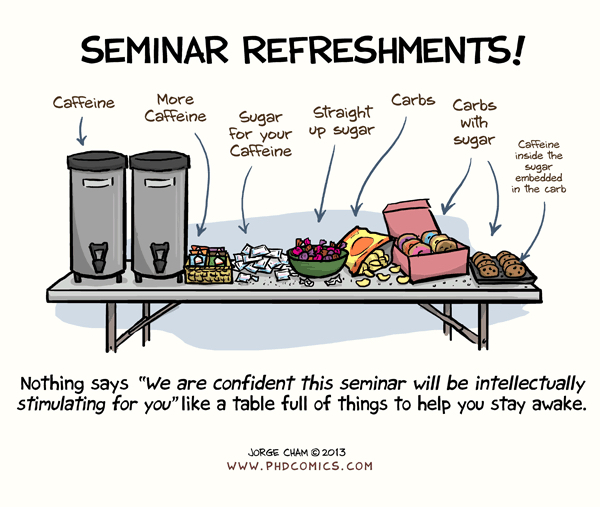
\includegraphics[width=3.2in]{phdRefreshments}\\
     
     \LARGE{Receso}
 \end{frame}
%=*=*=*=*=*=*=*=*=*=*=*=* 
\subsection{Preparando un artículo}
%Después del receso
 \begin{frame}
   \frametitle{Submitting - Envió de artículos}
   \begin{columns}
     \column{0.5\textwidth}
     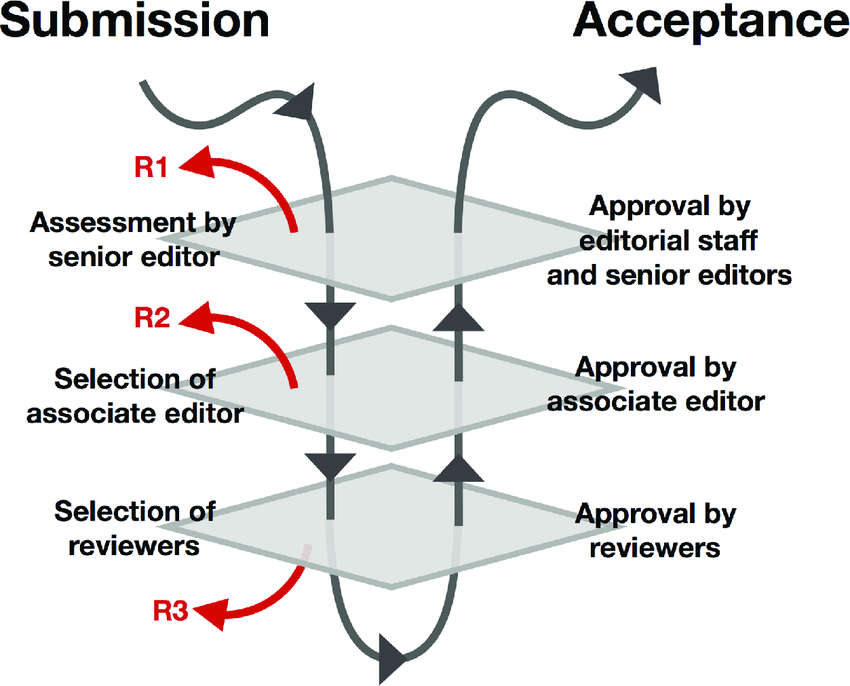
\includegraphics[width=2.5in]{peer-review}
     \column{0.5\textwidth}
     \begin{itemize}
     \item<1-> Definir el tipo de artículo:
       congreso, capítulo, \textit{review},
       \textbf{JCR}, \textit{open-access}.
     \item<2-> Revisar lineamientos o guías:
       cada editorial tiene sus propias
       reglas y requisitos.
     \item<3-> Definir las secciones: en
       función de la editorial. 
     \end{itemize}
   \end{columns}
 \end{frame}
%+++++++++++++++++++
 \begin{frame}
   \frametitle{Selecccionando el tipo de
     artículo}
   \begin{columns}
     \column{0.5\textwidth}
     
\includegraphics[width=2.5in]{elsevier-logo}
     \column{0.5\textwidth}
     \begin{itemize}
     \item<1-> \textbf{Regular papers}: Theoretical
       foundations and empirical evidence to
       make a scientific contribution.
     \item<2-> \textbf{Review essays}:
       authoritative reviews of the
       literature, offering an updated and
       critical discussion of the state of
       the art.
     \item<3-> \textbf{Methodological insights}:
        on novel methods and significant
       improvements to conventional
       techniques
     \end{itemize}
   \end{columns}
 \end{frame}
%+++++++++++++++++++
 \begin{frame}
   \frametitle{Líneamientos editoriales}
   \begin{columns}
     \column{0.5\textwidth}
     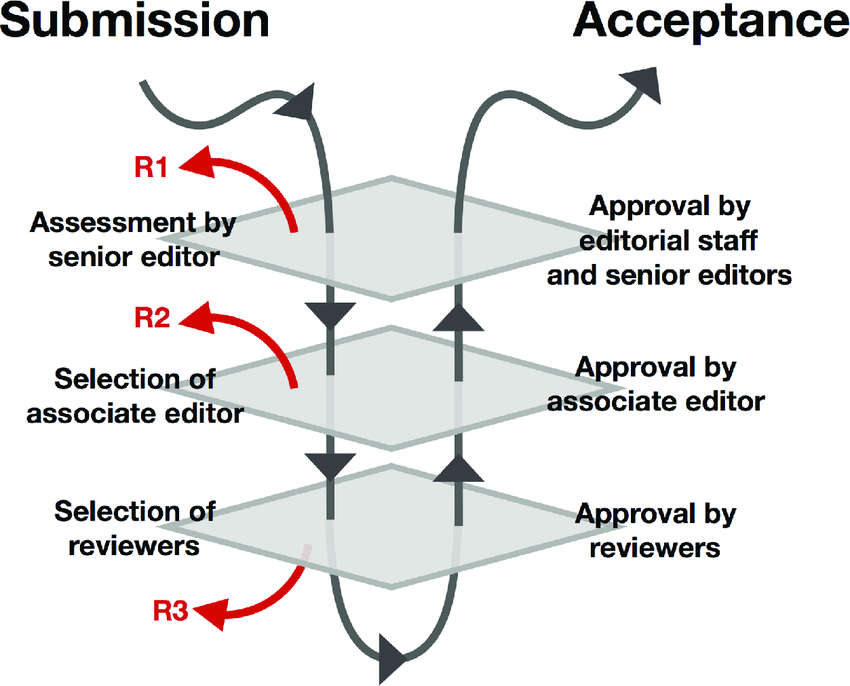
\includegraphics[width=2.5in]{peer-review}
     \column{0.5\textwidth}
     \centering
     \href{../material/elsevier/1385-8947.pdf}{
       Chemical Engineering Journal \\
       Author Information Pack} 
   \end{columns}
 \end{frame}
%+++++++++++++++++++
 \begin{frame}
   \frametitle{Definición de las secciones}
   \begin{columns}
     \column{0.5\textwidth}
     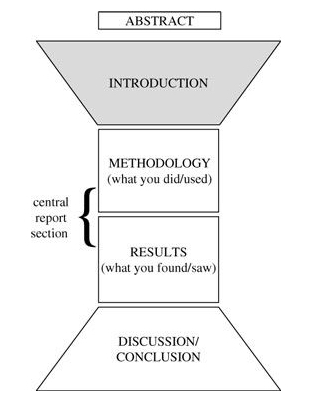
\includegraphics[width=2.in]{structure}
     \column{0.5\textwidth}
     \begin{itemize}
     \item<1->Las secciones son normalmente
       las mismas en las editoriales
     \item<2->No deben de pasar de entre 5 a 7
       hojas, dos columnas
     \item<3-> Las imágenes son en blanco y
       negro
     \item<4->Contenido del artículo en texto
       plano e imágenes por separado
     \item<5-> ¿Qué escribir primero y cómo? 
     \end{itemize}
   \end{columns}
 \end{frame}
%======= Día 2 =========
\section{Día 2: Sección Introducción }
% +++++++++++++++++++
\subsection{Revisando una introducción}
\begin{frame}[plain]
  \frametitle{Introducción de ejemplo}
  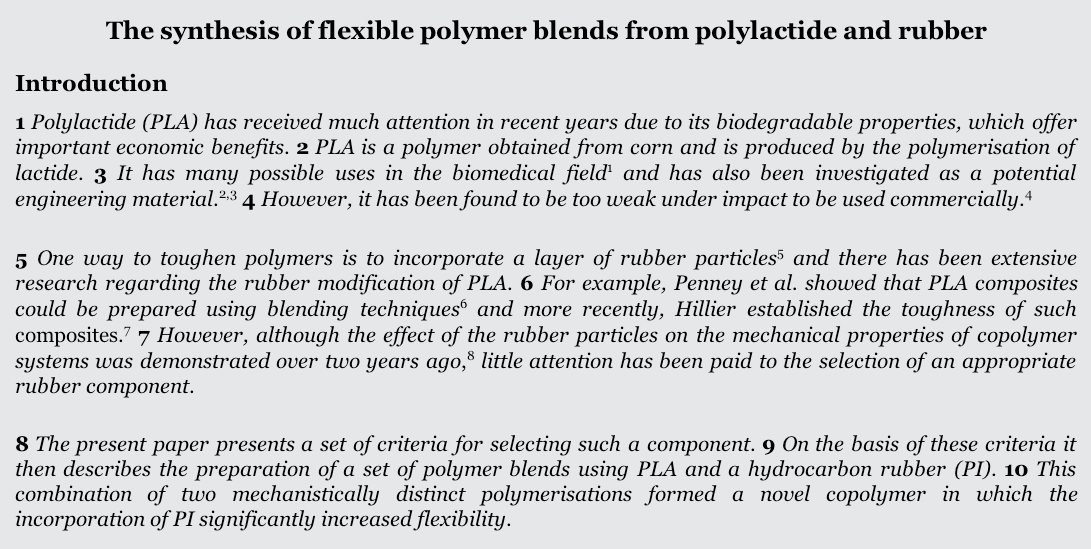
\includegraphics[width=4.5in]{1introduction}
\end{frame}

%+++++++++++++++++++
\begin{frame}[plain]
  
\includegraphics[width=4.5in]{meme-1}
\end{frame}
%+++++++++++++++++++
\subsection{Bibliografía}
\begin{frame}{Entorno bibliografía}
  El entorno \texttt{thebibliography} es
  nativo de \LaTeX{} y puede preferirse
  cuando el documento \textbf{contendrá pocas citas
  bibliográficas}(menos de 20) o será un documento que
  pasará por la revisión de diversos
  autores\cite[pág 21]{Mata2014}. En la
  siguiente sección de código se muestra el
  entorno \texttt{thebibliography}.
\end{frame}

%+++++++++++++++++++
\begin{frame}[containsverbatim]
\begin{lstlisting}[caption=Entorno ]
Preambulo
...
\begin{document}
...
\begin{thebibliography}{X}
\bibitem{clave1} Texto de la referencia 1.
\bibitem{clave2} Texto de la referencia 2.
\end{thebibliography}
\end{document}
\end{lstlisting}
  El argumento $X$ del entorno indica el
  número de entradas que habrá en el
  documento. Y cada entrada va acompañada del
  comando \texttt{$\backslash$bibitem}, el
  argumento (clave1) es una referencia para
  el usuario y se recomienda que sea el autor
  y el año, tal como se usa en el estilo de
  referencias tipo \textbf{Harvard}. El texto
  de la referencia debe usarse dependiendo
  del estilo de documento que se redacte.
\end{frame}
%+++++++++++++++++++

\begin{frame}[containsverbatim]
\frametitle{Citas bibliográficas}
Para hacer una cita bibliográfica debe usarse la instrucción \texttt{$\backslash$cite} con la etiqueta correspondiente.

\begin{lstlisting}[caption=Ejemplo de citas bibliográficas]
Como se puede ver en \cite{Mata2014} ...
...
Como se puede ver en \cite[pag 3]{Mata2014}...
\end{lstlisting}
\end{frame}

%+++++++++++++++++++

%+++++++++++++++++++
%+++++++++++++++++++
%+++++++++++++++++++
%+++++++++++++++++++
%Bibliography:
\begin{thebibliography}{10}

\bibitem{guiaLatex2014}[Nokyotsu, 2014]
http://nokyotsu.com.
\newblock LaTeX Fácil: Guía rápida de \LaTeX 

\bibitem{documentoLaTeX2014}[Guía de \LaTeX, 2014]
http://thales.cica.es
\newblock Guía para la configuración de documentos de \LaTeX.

\bibitem{Moser2013}[Moser, 2013]
\newblock How to typeset equations in \LaTeX.

\bibitem{Reckdahl2006}[Reckdahl K., 2006]
\newblock Using imported graphics in \LaTeX{} and PDF\LaTeX{}. 

\bibitem{Hunninger2012}[Hünninger D., 2012]
\newblock \LaTeX{} a Wikibook, www.wikibooks.org

\bibitem{Mata2014}[Mata-Pérez M., 2014]
\newblock Bibliografía en \LaTeX{}, una guía concisa de BIB\TeX{}. 

\end{thebibliography}

%+++++++++++++++++++

\end{document}